\frame
{
  \frametitle{A 排序大师 {by \itshape Itst}}
	用最少的 "段交换" 操作将长度为 $n$ 的排列排序。
	
	"段交换" 操作为以下操作:将排列分成五段,其中第二段和第四段不能为空、其他段可以为空,交换第二段和第四段再拼回去。

	$n\le 2000$.
}

\begin{frame}{正解}

	需要最小化交换次数,意味着我们同时需要上界和下界的分析.

	下界分析的常用办法是图模型,最常见的是 $p_i\rightarrow i$ 的模型. 但对于这个操作来说它不适用,因为一次交换会导致图上很多的边产生改变. \pause

	这提示我们需要考虑这样的图模型:在这个模型下,一次段交换操作只会改变其中常数条边.

	再注意到,一次交换中形如 $p_i\rightarrow p_{i+1}$ 的边只会改变最多四条,符合我们的要求,但这个模型并不能直接用于下界分析,因为目标状态是一条特殊的链,不能用环数分析.

\end{frame}

\begin{frame}{正解}

	我们做一些简单的调整:在排列最前面加入一个 $0$、最后加入一个 $n+1$,然后加入 $p_i\rightarrow p_{i+1}$ 的边。此时终态是一个 ${n+1}$ 个自环构成的图,符合“单次操作改变边数少”,同时环数相关的下界分析可以利用了.

	此时我们来考虑一次操作究竟会干什么.

\end{frame}

\begin{frame}{正解}
	不妨假设第三段非空,此时交换前后的状况如下:

	\centering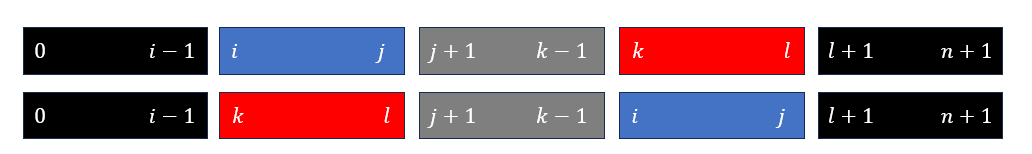
\includegraphics[width=\textwidth,keepaspectratio]{sources/A1.jpg}

	最初的四条边


$p_{i-1}+1\rightarrow p_i, p_j+1\rightarrow p_{j+1}, p_{k-1}+1\rightarrow p_k, p_l+1\rightarrow p_{l+1}$

 	被改为

$p_{i-1}+1\rightarrow p_k, p_l+1\rightarrow p_{j+1}, p_{k-1}+1\rightarrow p_i, p_j+1\rightarrow p_{l+1}$

	看起来还是画图比较直观(

\end{frame}


\begin{frame}{正解}

	\centering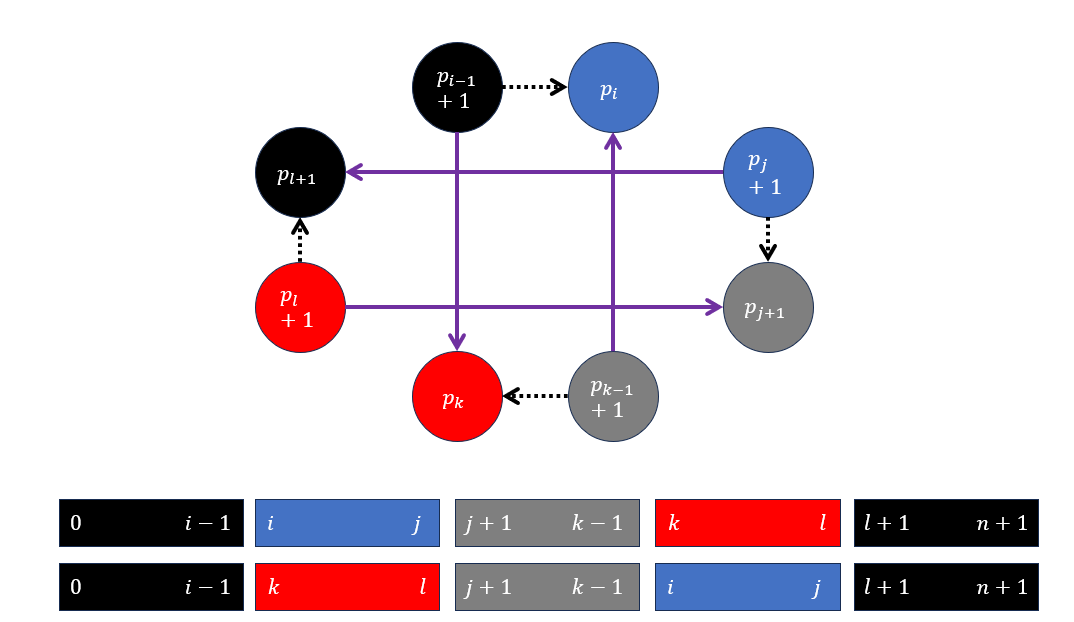
\includegraphics[width=\textwidth,keepaspectratio]{sources/A2.jpg}

\end{frame}

\begin{frame}{正解}

	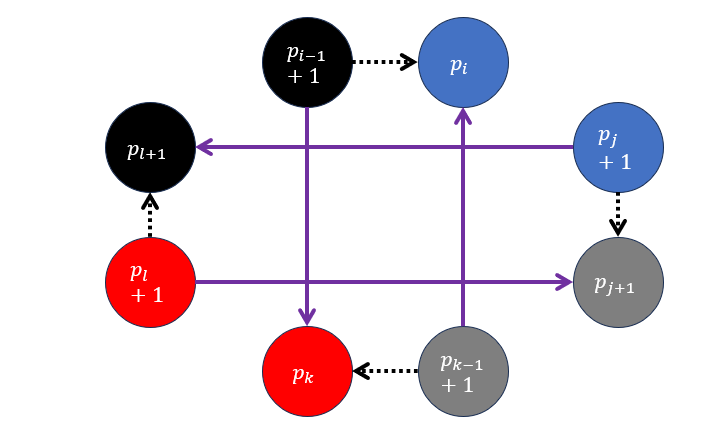
\includegraphics[width=0.8\textwidth,keepaspectratio]{sources/A3.jpg}

	这个修改操作相当于做以下操作两次:

	\begin{itemize}
	\item 选两条边交换它们的出点
	\end{itemize}

	这个操作会恰好将环数改变 \texttt{1}(读者自证不难),因此一次操作最多将环数减少 \texttt{2},且不会改变环数的奇偶性。

\end{frame}

\begin{frame}{正解}

	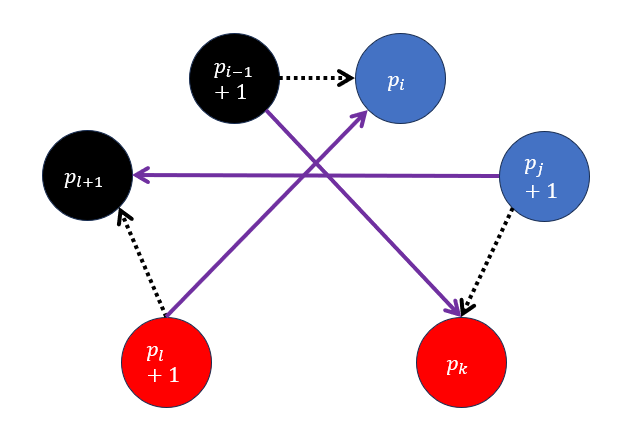
\includegraphics[width=0.8\textwidth,keepaspectratio]{sources/A4.jpg}

	对于第三段为空($j+1=k$)的情况,可以认为是先交换了 $p_{i-1}+1$ 和 $p_j+1$ 的出边,再交换 $p_j+1$ 和 $p_l+1$ 的出边,所以环数也最多改变不超过 \texttt{2},且不改变环数奇偶性。

\end{frame}

\begin{frame}{正解}

	因此我们只要能找到一种操作方案每次将环数增加 2 就行了。

	考虑如下构造:

	 \begin{enumerate}
	\item 选择一个最小的 $x$ 满足 $x$ 前面有比 $x$ 大的元素
	\item 再选择 $x$ 前面最大的元素 $y$
	\item 此时 $x-1$ 一定在 $y$ 前面(否则与 $x$ 的最小性矛盾),且 $y+1$ 一定在 $x$ 后面(否则与 $y$ 的最大性矛盾),因此用一次操作将 $x-1,\cdots, y, \cdots, x, \cdots, y+1$ 变为 $x-1, x, \cdots, y, y+1$
	\end{enumerate}

\end{frame}

\begin{frame}{正解}

	在  $x-1,\cdots, y, \cdots, x, \cdots, y+1$  中被修改的四(或三)条边为与 $x$ 相邻的两条边和与 $y+1$ 相邻的两条边,所以这四(或三)条边一定在一个或两个环里.

	而修改过后,出现了额外的两个自环($x-1, x$ 以及 $y, y+1$)。因为环数奇偶不会改变,因此环数一定加 \texttt{2}. \pause

	\sout{当然也有一些其他的构造可能满足以上条件.}\\ \sout{所以这题正确的做法是,猜一堆结论,写个 gen 拍一拍,拍过了就交.}


\end{frame}